%
% Complete documentation on the extended LaTeX markup used for Insight
% documentation is available in ``Documenting Insight'', which is part
% of the standard documentation for Insight.  It may be found online
% at:
%
%     http://www.itk.org/

\documentclass{InsightArticle}

\usepackage{color}

% to be able to use options in graphics
\usepackage{graphicx}
% for pseudo code
\usepackage{listings}
% subfigures
\usepackage{subfigure}

% some maths symbols
\usepackage{amstext,amssymb}

% to include accents in bliblio
\usepackage[T1]{fontenc}
\usepackage[latin1]{inputenc}


% to be able to use options in graphics
\usepackage{graphicx}
% for pseudo code
\usepackage{listings}
% subfigures
\usepackage{subfigure}
\usepackage{pseudocode}

 \definecolor{lightgray}{gray}{.75}
\newcommand{\commentaire}[1]{
\colorbox{lightgray}{#1}
}

\let\oldtabular=\tabular
\def\tabular{\small\oldtabular}

%%%%%%%%%%%%%%%%%%%%%%%%%%%%%%%%%%%%%%%%%%%%%%%%%%%%%%%%%%%%%%%%%%
%  hyperref should be the last package to be loaded.
%%%%%%%%%%%%%%%%%%%%%%%%%%%%%%%%%%%%%%%%%%%%%%%%%%%%%%%%%%%%%%%%%%
\usepackage[
bookmarks,
bookmarksopen,
backref,
colorlinks,linkcolor={blue},citecolor={blue},urlcolor={blue},
]{hyperref}

%  This is a template for Papers to the Insight Journal. 
%  It is comparable to a technical report format.

% The title should be descriptive enough for people to be able to find
% the relevant document. 
\title{Efficient N-Dimensional surface estimation using Crofton formula and run-length encoding}

% Increment the release number whenever significant changes are made.
% The author and/or editor can define 'significant' however they like.
% \release{0.00}

% At minimum, give your name and an email address.  You can include a
% snail-mail address if you like.
\author{Ga\"etan Lehmann$^{1,2}$ {\small{and}} David Legland$^{3,4}$}

\authoraddress{\small{
{$^1$}INRA, UMR 1198 Biologie du D\'eveloppement et Reproduction, Jouy-en-Josas, F-78350, France\\
{$^2$}ENVA, UMR 1198 Biologie du D\'eveloppement et Reproduction, Jouy-en-Josas, F-78350, France\\
{$^3$}INRA, UMR 0782 G\'enie et Microbiologie des Proc\'ed\'es Alimentaire, Thiverval-Grignon, F-78850, France\\
{$^4$}AgroParisTech, UMR 0782 G\'enie et Microbiologie des Proc\'ed\'es Alimentaire, Thiverval-Grignon, F-78850, France\\
}}

\begin{document}
\maketitle

\ifhtml
\chapter*{Front Matter\label{front}}
\fi


\begin{abstract}
\noindent
Unlike the measure of the area in 2D or of the volume in 3D, the perimeter and the surface are not easily measurable in a discretized image.
In this article we describe a method based on the Crofton formula to measure those two parameters in a discritized image. The accuracy of
the method is discussed and tested on several known objects. An algorithm based on the run-length encoding of binary objects is presented
and compared to a brute force approach.
An implementation is provided and integrated in the LabelObject/LabelMap framework contributed earlier by the authors.
\end{abstract}

\tableofcontents

\section{Introduction}

Surface area and perimeter are widely used parameters describing the size of objects observed in images, 
and are commonly used for computing various shape factors.
Unlike the area that can be easily measured by counting pixels belonging to the object, measuring the 
perimeter is not as straightforward, 
and naive methods can lead to huge systematic errors \cite{Klette2004, Legland2007}.
Usually, the countour of the object is extracted, then its length is measured.
The same approach is usually applied to 3D images: the boundary of the 3D object is first reconstructed,
e.g. by using marching cubes \cite{Lorensen1987}, then its surface area is computed by summing 
area of individual triangles.

The Crofton method is an alternative method that allows estimating the perimeter of 2D objects,
the surface area of 3D objects, and more generally the $(d-1)$-dimensional measure of $d$-dimensional 
object boundary. 
It is based on counting intercept number of the object boundary with a set of isotropic test lines, 
and provide an unbiased estimate of the actual perimeter or surface.

The article first recalls the mathematical principles of $d$-perimeter measures in digital images
using the Crofton method. An efficient implementation based on run-length encoding is then presented.
The method is evaluated on various $2D$ and $3D$ synthetic shapes and compared with other methods.
The effect on the roundness shape factor is also investigated.


\section{Principles}
\subsection{Surface area and perimeter estimation}

% Crofton formula
Perimeter measure of 2D objects, surface area measure of 3D objects 
and more generally $(d-1)$-surface measure of $d$-dimensional objects 
can be expressed in a unified formalism by using the Crofton formula.
This formula consists in integrating the intercept number of the object with
lines of various orientation and positions. Its expression in
the general form is:
\begin{eqnarray}
S^{(d-1)}(X) & = & \frac{d \cdot v_d}{v_{d-1}}\int_{\mathcal{L}^d}\chi\left(X\cap L\right) dL
\end{eqnarray}
where $X$ is the structure of interest, $v_d$ is the volume of the $d$-dimensional ball,
$\mathcal{L}^d$ is the set of all lines in the $d$-dimensional space. 
The above integral is normalised such that the mass of lines hitting the unit ball 
equals $v_{d-1}$, the measure of the unit ball projection on a $(d-1)$-dimensional plane.

The Euler-Poincar\'e characteristic $\chi$ is equal to number of connected components
of the intersection of $X$ with a line $L$, or equivalently half the number of intersections
of the boundary of $X$ with the line.

% 2D and 3D
For planar and 3D cases, Equation 1 can be rewritten:
\begin{eqnarray}
P(X) & = & \pi \int_{\mathcal{L}^2} \chi \left( X \cap L \right) dL \\
S(X) & = &  4  \int_{\mathcal{L}^3} \chi \left( X \cap L \right) dL
\end{eqnarray}

\subsection{Crofton formula in discrete images}

The Crofton formula can be easily applied to discrete binary images \cite{Lang2001, Legland2007}. 
The integral over lines can be decomposed into an integral over a finite set of directions
and an integral over all the lines parallel to a given direction. 

For the planar case, the perimeter can be estimated by considering horizontal and vertical lines, 
i.e.\ two directions. An alternative is to use the diagonals, resulting in four directions. 
Perimeter estimate is then written as:
\begin{eqnarray}
P(X) & \simeq & \pi \sum_{k}\frac{c_{k}}{\lambda_{k}}\chi \left( X \cap L_{k} \right)
\end{eqnarray}
where $c_k$ is the discretization weight associated to direction $k$, 
$\lambda_k$ is the density of discrete lines in direction $k$, 
and $L_k$ is the set of all discrete lines in direction $k$.

The line density $\lambda_k$ may vary according to the directions, 
due to image resolution or to the use of diagonals. 
It is computed as the ratio of the distance between two neighbor pixels with
the area associated to a pixel.
When only horizontal and vertical directions are used, associated weights $c_k$ equal $1/2$.
When diagonals are used, weights are obtained by projecting direction vectors on the unit circle, 
and by computing the relative fraction of circle associated to each direction 
(Fig.~\ref{fig:DirectionWeights2D3D}).

% Compute direction weights
\begin{figure}[!htb]
\begin{center}
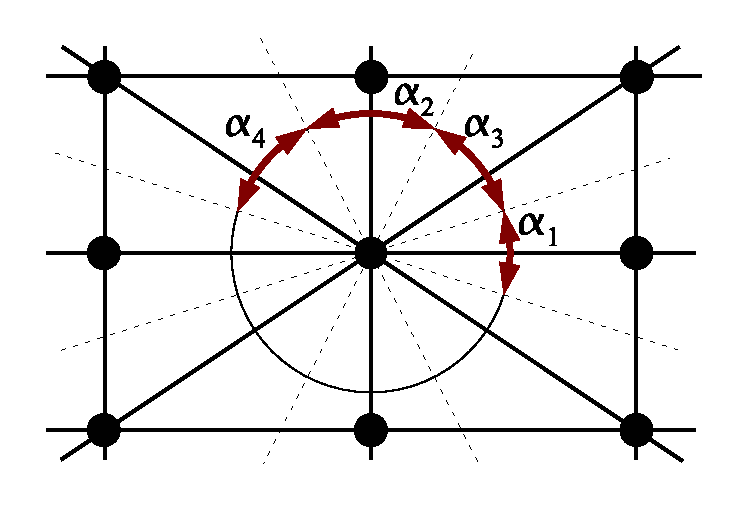
\includegraphics[width=8cm]{images/directionWeights2D}
\includegraphics[width=7cm]{images/directionWeights3D_335}
\end{center}
\caption{Computation of direction weights for rectangular grids. 
Left: planar case. Black dots correspond to pixel centers. 
Angular regions are computed between direction bisectors.
Right: 3D case. The unit sphere is partitioned into spherical polygons
corresponding to each of the 26 oriented directions.
}
\label{fig:DirectionWeights2D3D}
\end{figure}

In a similar way, surface area of $3D$ objects may be estimated using following approximation:
\begin{eqnarray}
S(X) & \simeq & 4\sum_{k}\frac{c_{k}}{\lambda_{k}}\chi \left( X \cap L_{k} \right)
\end{eqnarray}
where $L_k$ is the set of $3D$ discrete lines parallel to direction $k$, 
$c_k$ the discretization weight associated to $3D$ direction $k$, 
and $\lambda_k$ the density of discrete lines in direction $k$.

Line densities are computed as for the planar case, by dividing distance of neighbor
voxels in direction $k$ by the volume associated to a single voxel.
When surface area is estimated by taking into account the three main direction in images, 
associated weights $c_k$ equal $1/3$. If more directions are considered, the strategy of
Ohser and M\"ucklich \cite{Ohser2000} was applied: each direction was projected on the unit sphere, 
and was used as a germ for computing Voronoï diagram on the unit sphere. 
The relative surface area of each spherical domain was used as weight for the
corresponding direction (Fig.~\ref{fig:DirectionWeights2D3D}).

\subsection{Intercepts count in digital images}

The number of connected components in the intersections of the structure with a discrete line
is obtained by counting the number of intercepts with its boundary.
This intercepts count can be efficiently computed by using the run-length
encoding of the binary objects.

The run-length encoding groups all the pixels on the same line in a single element. If the binary object is compact enough, as it is often the case for connected components, the run-length encoding heavily reduces the number of elements required to represent the object, compared to the simple pixel representation. Thanks to the run-length encoding, it is possible to compute the intercepts the binary object line by line, instead of computing it pixel by pixel.

The data structure used as the input of the algorigthm is a set of all the indexes of the object with their first element remove -- in 3D, this is all the possible (y, z) pairs -- to which are associated a list of lines. The lines are coded as a $x$ position and a length.

The algorithm used to count the intercepts is described in Figure \ref{interceptCountAlgo}.

\begin{figure}[htbp]
\centering
\small
\begin{pseudocode}[framebox]{countIntercept}{O}
\COMMENT{intercept count} \\
ic \GETS \emptyset \\
\COMMENT{the offset of the neighbors on the first axis} \\
xno \GETS offset(0) \\
xno[0] \GETS 1 \\
\FOREACH ls \in O \DO
\BEGIN
  \COMMENT{2 intercepts per line on the first axis} \\
  ic[xno] \GETS ic[xno] + 2 \cdot length(ls) \\
  \FOREACH nls \in neighbors(ls) \DO
  \BEGIN
    \COMMENT{straight and diagonal offsets of the neighbors} \\
    no \GETS offset(nls) \\
    dno \GETS offset(nls) \\
    dno[0] \GETS 1 \\
    \IF isEmpty(nls) \THEN
    \BEGIN
      \COMMENT{all the lines are on a contour} \\
      \FOREACH l \in ls \DO
      \BEGIN
    ic[no] \GETS ic[no] + length(l)\\
    ic[dno] \GETS ic[dno] + 2 \cdot length(l)
      \END
    \END
    \ELSE
    \BEGIN
      \COMMENT{iterate over the lines in $ls$ and the empty lines in $nls$} \\
      il \GETS iterator(ls) \\
      inl \GETS iterator(nls) \\
      nMin \GETS -\infty \\
      nMax \GETS pos(inl) - 1 \\
      \WHILE isNotAtEnd(il) \DO
      \BEGIN
        lMin \GETS pos(il) \\
        lMax \GETS pos(il) + length(il) - 1 \\
        \COMMENT{measure the intersection of these two lines} \\
    ic[no] \GETS ic[no] + max( 0, min( lMax, nMax ) - max( lMin, nMin ) + 1 ) \\
    ic[dno] \GETS ic[dno] + max( 0, min( lMax, nMax+1 ) - max( lMin, nMin+1 ) + 1 )\\
    ic[dno] \GETS ic[dno] + max( 0, min( lMax, nMax-1 ) - max( lMin, nMin-1 ) + 1 )\\
        \COMMENT{and move to the next line, either in $ls$ or in $nls$} \\
    \IF nMax \leq lMax \THEN
    \BEGIN
          nMin \GETS pos(inl) + length(inl) \\
          next(inl) \\
          \IF isNotAtEnd(inl) \DO
            nMax \GETS pos(inl) - 1
          \ELSE
            nMax \GETS \infty
    \END
    \ELSE
          next(il)
      \END
    \END
  \END
\END
\end{pseudocode}
\caption{\label{interceptCountAlgo}The algorithm used to count the intercepts}
\end{figure}


\subsection{Roundness}

The roundness is defined as the ratio of equivalent $d$-perimeter over the measured $d$-perimeter. 
The equivalent $d$-perimeter is defined as the perimeter of the $d$-ball with same volume $V$.
\begin{eqnarray}
roundness             & = & \frac{P_{eq}}{P} \\
P_{eq}                & = & \frac{d \cdot V_{eq}}{R_{eq}} \\
R_{eq}                & = & \sqrt[\displaystyle d]{\frac{V\cdot\Gamma(\frac{d+1}{2})}{\pi^\frac{d}{2}}} \\
\Gamma(\frac{d+1}{2}) & = & \begin{cases}
                               \displaystyle \frac{d}{2}!  &\text{if}~ d ~\text{is even} \\
                               \displaystyle \frac{\sqrt{\pi} \cdot d!!}{2^{\frac{d+1}{2}}}  &\text{if}~ d ~\text{is odd} \\
                            \end{cases} \\
d!!                   & = & \begin{cases}
                                1 &\text{if}~ d \leq 1 \\
                                d \cdot (d-2)!!  & \text{otherwise} \\
                             \end{cases}
\end{eqnarray}


Roundness takes values between $0$ and $1$. 
It is equal to $1$ for circular or spherical shapes, 
and decreases for more complicated shapes.


\section{Implementation}

The implementation of this algorithm has been done in the \verb$itk::ShapeLabelMapFilter$ class, which is already in charge of the computation of
several shape descriptors. The run-length encoding used in the \verb$itk::LabelObject$ representation is reused.
The implementation is N-dimensional and thus is usable for any image dimension. The most useful cases, 2D and 3D have been specialized
to provide a more accurate estimation by also using the diagonals -- 4 directions in 2D and 13 directions in 3D. In the 4D case and greater,
the diagonals are not used.

The perimeter estimation is now turned on by default, but can still be disabled with \verb$SetComputePerimeter(false)$ in
\verb$itk::ShapeLabelMapFilter$ if not needed. This should enhance the user experience, especially for the attributes non obviously derived
from the perimeter like the roundness.

\subsection{N-Dimensional name}
The attribute is called {\em Perimeter} independently of the dimension of the image and is available in the \verb$itk::ShapeLabelObject$.

\subsection{Border management}

The borders of the image is considered to be in the background, so the contour of an object touching the border of the image is measured.
This was not the case in the previous (undocumented) implementation and has been proven to be misleading for many users.
It is possible to subtract the perimeter on the border to the full perimeter if the measure without the part touching the border is needed.

\subsection{Multithreading}

The architecture implemented in \verb$itk::ShapeLabelMapFilter$ use one thread per LabelObject. The perimeter estimation has been integrated in this
architecture, providing a multithreaded implementation as long as there are several LabelObjects in the input LabelMap.


\section{Evaluation method}

\subsection{Test shapes}

Perimeter and surface area are measured on discretization of various 2D and 3D shapes 
whose true perimeter or surface area is known.

Planar test shapes include disks, rings obtained by the difference of several disks,
trefoil shape, ellipses with $a=XX$ and $b=XX$, and rectangle with length $XX$ and width $XX$.

Test shapes for 3D measurements include
balls with various radii, hollow ball, prolate and oblate ellipsoids, and cuboids. 
For each type of shape, several orientations were considered.

Shapes were discretized following the Gauss discretization scheme \cite{Klette2004, Legland2007}.
Binary images can be considered as a subset of a rectangular grid $L_d$ where
d = 2,3. Such a grid can be written as
\begin{eqnarray}
L_d = \Delta_{1} \mathbb{Z} \times \ldots \times \Delta_{1} \mathbb{Z},
\end{eqnarray}
where the $d$-uple $(\Delta_{1},\ldots,\Delta_{d})$ defines the pixel
or voxel size. 
A grid point $x$ belongs to the reconstructed structure if the grid
cell centered on $x$ hits $X$ (See Fig.~\ref{fig:DiskDiscretization}).

% Example of reconstruction of a discrete disk
\begin{figure}[!htb]
\begin{center}
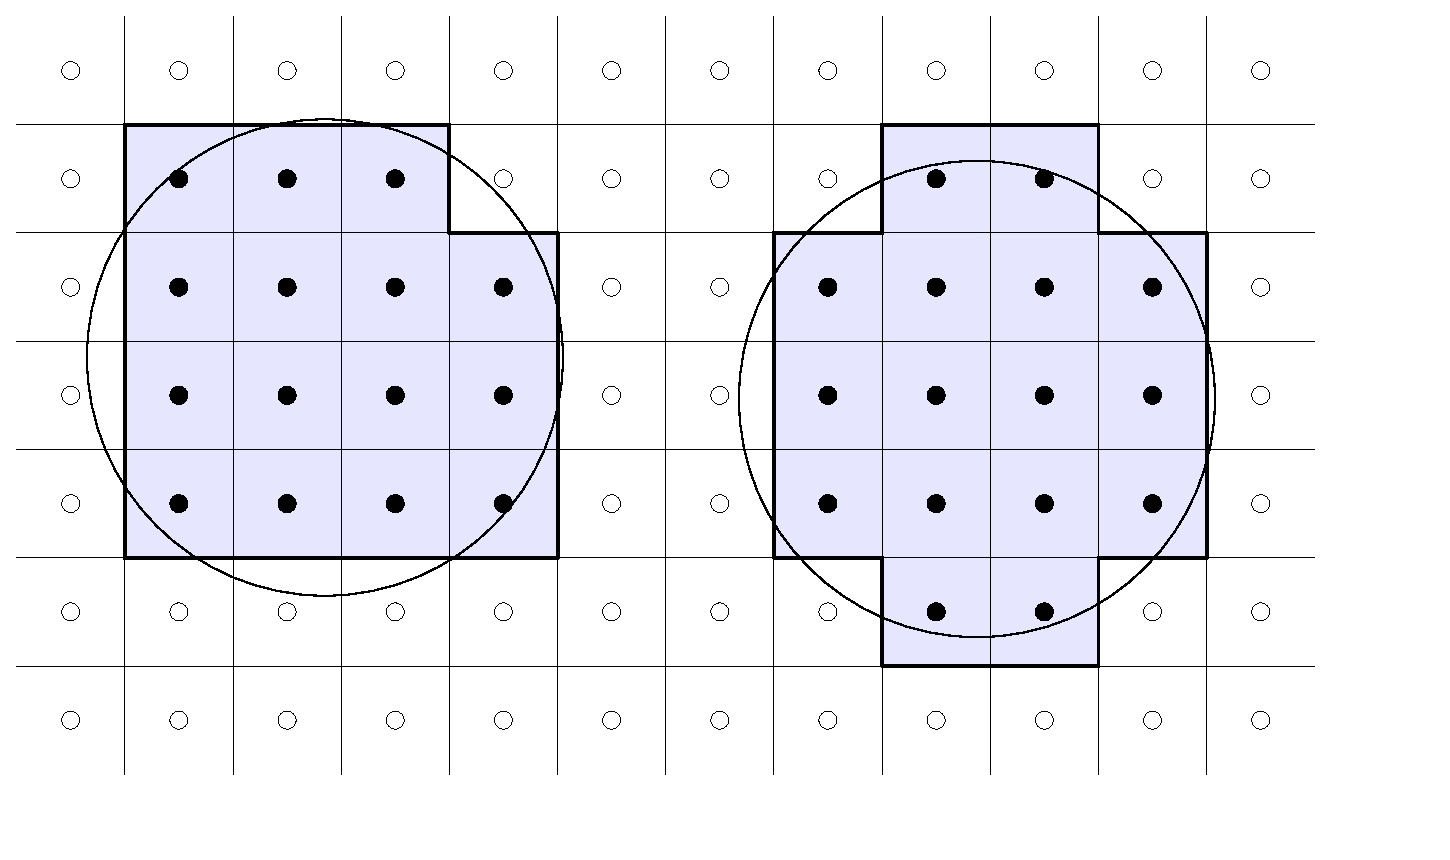
\includegraphics[width=12cm]{images/discreteDisks2}
\end{center}
\caption{Discretization of two disks with same radius and different positions. 
A grid cell belong tho the reconstructed shape if its center is inside the original shape.
The reconstructed shapes have different size and shape.}
\label{fig:DiskDiscretization}
\end{figure}


\subsection{Measurements}

For each test shape, measurements were made on
several discretisation of the shape, with various orientations and various origins.
The center of each shape was chosen at random within the center pixel or voxel of the grid.

Perimeter of 2D discretized shapes was measured using Crofton method using 2 and 4 directions, 
and by computing the length of the reconstructed contour (Matlab Software was used).
Surface area of 3D discretized shapes was measured using Crofton method using 3 and 13 directions, 
and by computing the surface area of the reconstruced shape obtained by the marching cubes algorithm.
The average and the standard deviation of measurements were computed for all shapes discretized
with the same resolution. Effect of orientation was investigated by computing average and standard 
deviation of shapes having the same orientation.

% \subsection{Timing evaluation}
% ???

\section{Accuracy}

\subsection{Perimeter of disks at various resolutions}

Figure \ref{fig:MeasureDiskPerimeter} shows average and standard deviation of perimeter
measured on disks with various resolutions. Perimeter measured using Crofton method converges
towards the real value when the resolution increase. 
The convergence speed is faster when four directions are used instead of two, 
and the variability is lower.

% Example of reconstruction of a discrete disk
\begin{figure}[!htb]
\begin{center}
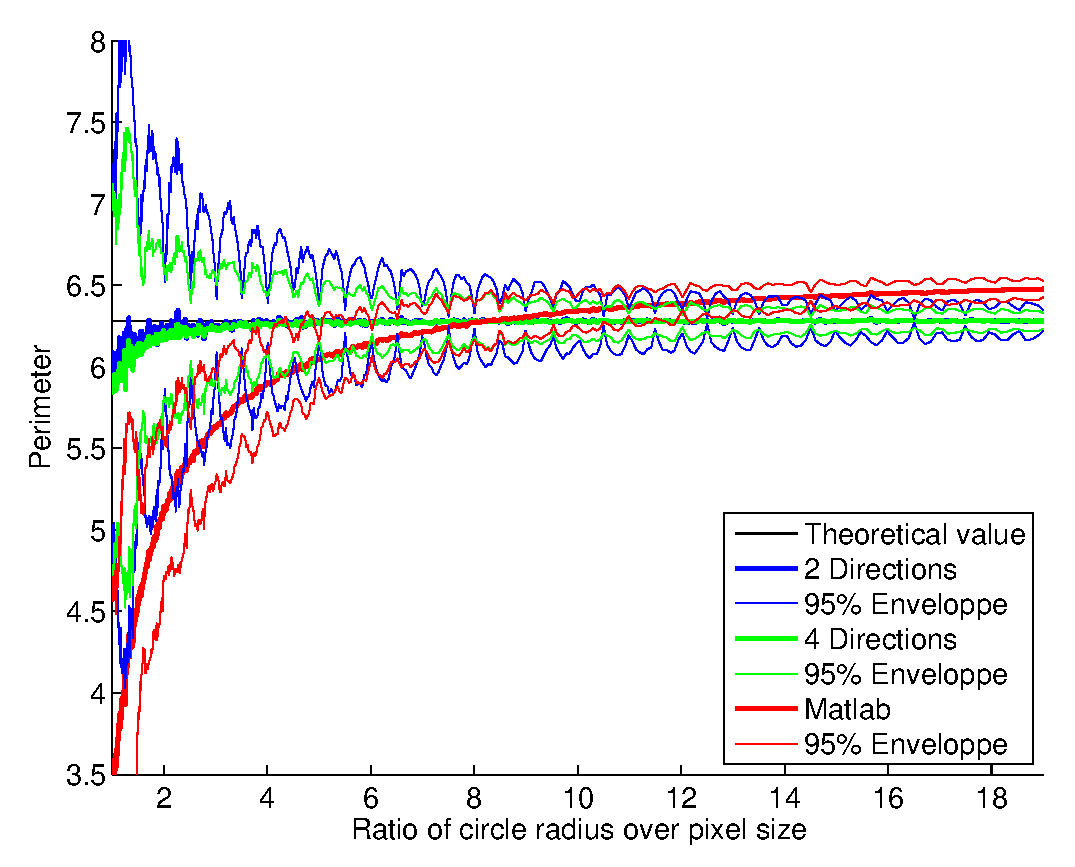
\includegraphics[width=10cm]{images/perimeterDisks}
\end{center}
\caption{Perimeter measure of disks with various resolutions and at random positions}
\label{fig:MeasureDiskPerimeter}
\end{figure}

Perimeters measured with Matlab show similar variability, but the measured values do not
converge toward the true value. This shows the inaccuracy of the method consisting in
counting boundary pixels.

The oscillations of the variability is due to the fact that for disks with diameters equal to an
integer, the number of intersections with horizontal or vertical lines is always the same, 
thus greatly reducing the variability of measures. 

\subsection{Perimeter of squares with various orientations}

Figure \ref{fig:MeasureSquareOriented} shows measures obtained on discretized squares (side 30 pixels)
with various orientations. All methods oscillate around the expected value. 
Using Crofton method with only 2 directions can produce greater errors on the measure than with 4 
directions. However, in both cases, the average over the orientations of the mean values is very close 
to the actual perimeter.

% Example of reconstruction of a discrete squares with various orientations
\begin{figure}[!htb]
\begin{center}
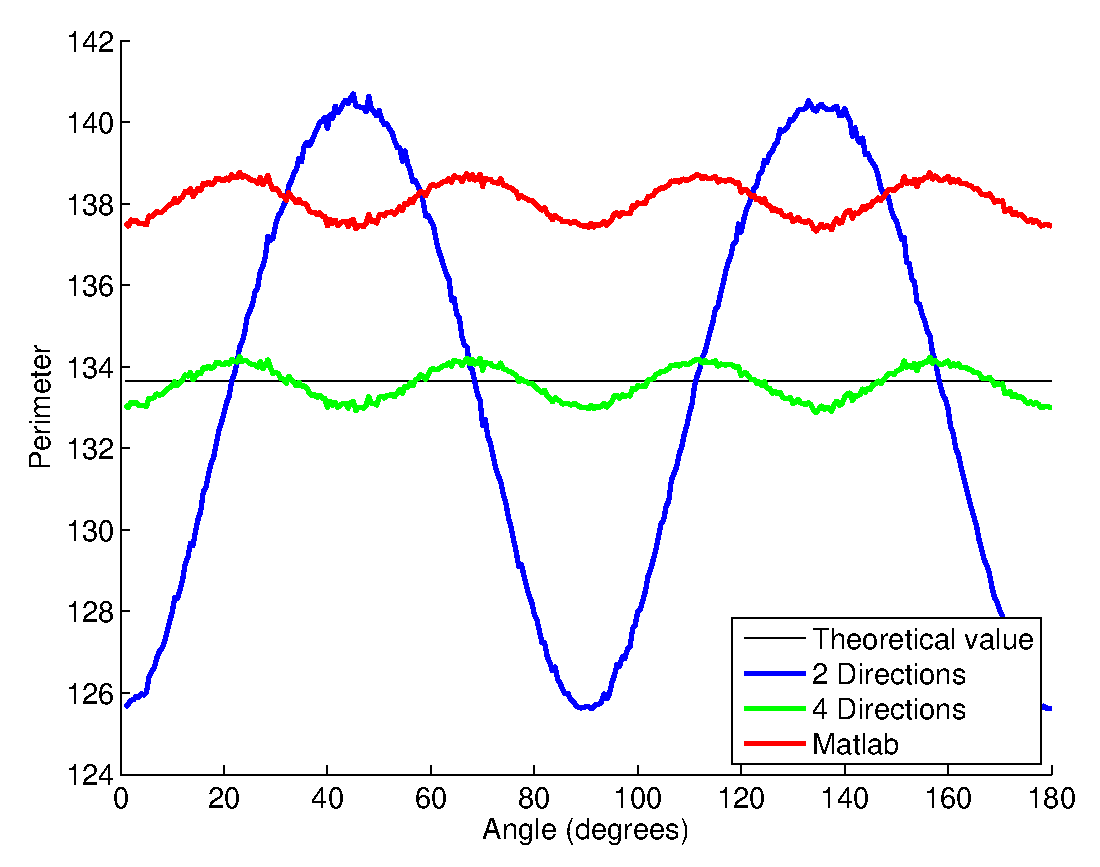
\includegraphics[width=8cm]{images/perimRotatedEllipses}
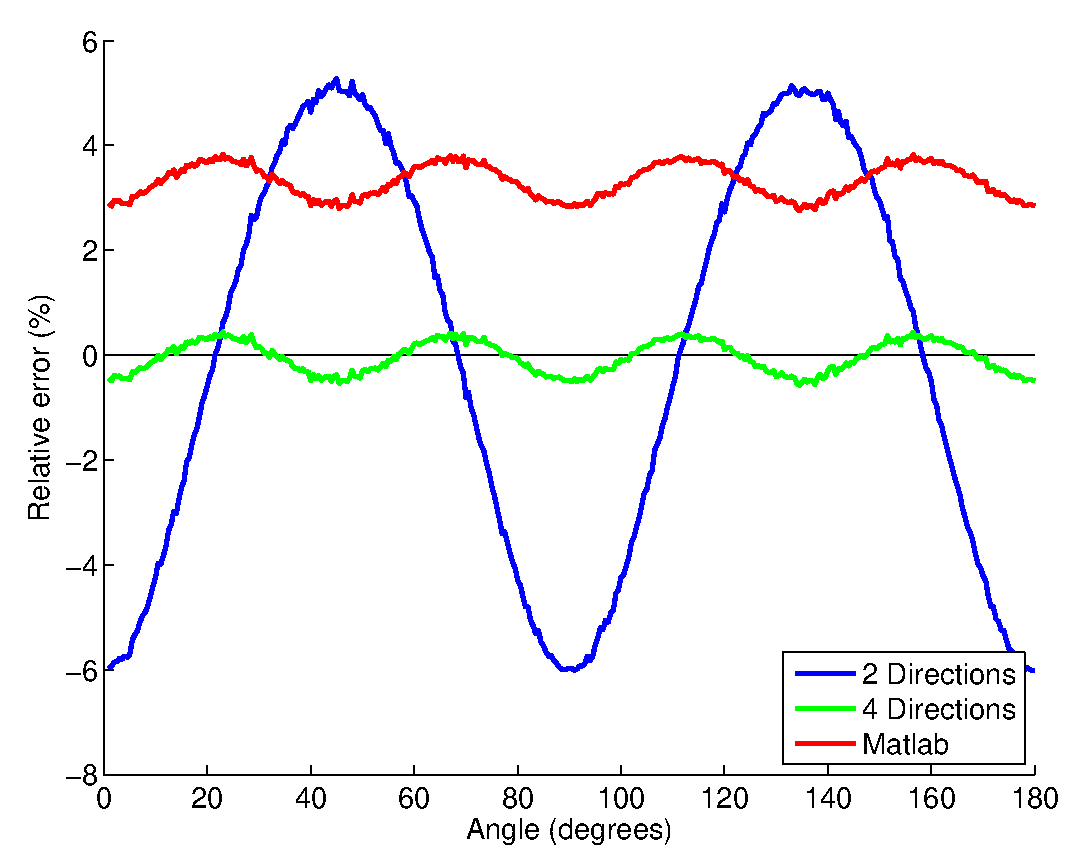
\includegraphics[width=8cm]{images/errorRotatedEllipses}
\end{center}
\caption{Variations of perimeter measure of a digitized ellipse depending on the orientation. 
Left: perimeter measures. Right: relative errors (in percent).}
\label{fig:MeasureSquareOriented}
\end{figure}


% TODO mesure pour des formes 3D
% able

\subsection{Surface area of 3D shapes}

Comarison of surface area measured on several discrete reconstructed shapes is given in
Table \ref{tab:CompareSurfaceArea}.
As for the planar case, the measure is closer to the actual value when using more
directions. The error is around 2 percent in average for 3 directions, and less than
1 percent for 13 directions.

When using isosurface reconstruction, the surface area is systematically over estimated.
The difference is around 8 percent in average.

\begin{table}[!htb]
\begin{center}\begin{tabular}{ccccccc}
Shape      & $(\varphi,\theta)$ & $S$            & $S_{crofton^3}$     & $S_{crofton^{13}}$  & $S_{VTKmarch}$       & $S_{ITKiso}$  \tabularnewline
\hline 
\hline 
ball       & $n.a.$             &     $11309.8$  & $11312.0\ (+0.0\%)$ & $11306.6\ (-0.0\%)$ & $12298.2\ (+8.7\%)$  & $12299.5\ (+8.8\%)$ \tabularnewline 
prolate    & $( 0,  0)$         &     $3082.9$   & $2938.7\ (-4.7\%)$  & $3084.6\ (+0.1\%)$  & $3354.1\ (+8.8\%)$   & $3354.9\ (+8.8\%)$  \tabularnewline
-          & $(45,  0)$         &     $-$        & $3137.3\ (+1.8\%)$  & $3086.3\ (+0.1\%)$  & $3353.9\ (+8.8\%)$   & $3354.7\ (+8.8\%)$  \tabularnewline
-          & $(45, 45)$         &     $-$        & $3150.6\ (+2.2\%)$  & $3083.3\ (+0.0\%)$  & $3351.5\ (+8.7\%)$   & $3352.2\ (+8.7\%)$  \tabularnewline
oblate     & $( 0,  0)$         &     $6856.8$   & $6290.7\ (-8.3\%)$  & $6807.6\ (-0.7\%)$  & $7410.2\ (+8.1\%)$   & $7411.3\ (+8.1\%)$  \tabularnewline
-          & $(45,  0)$         &     $-$        & $6872.0\ (+0.2\%)$  & $6789.0\ (-1.0\%)$  & $7369.7\ (+7.5\%)$   & $7370.7\ (+7.5\%)$  \tabularnewline
-          & $(45, 45)$         &     $-$        & $7154.7\ (+4.3\%)$  & $6808.5\ (-0.7\%)$  & $7385.9\ (+7.7\%)$   & $7386.7\ (+7.7\%)$  \tabularnewline
torus      & $( 0,  0)$         &     $11843.5$  & $11417.3\ (-3.6\%)$ & $11792.9\ (-0.4\%)$ & $12826.6\ (+8.3\%)$  & $12828.7\ (+8.3\%)$ \tabularnewline
-          & $(45,  0)$         &     $-$        & $11809.3\ (-0.3\%)$ & $11766.8\ (-0.6\%)$ & $12787.4\ (+8.0\%)$  & $12789.3\ (+8.0\%)$ \tabularnewline
-          & $(45, 45)$         &     $-$        & $12086.0\ (+1.9\%)$ & $11822.4\ (-0.2\%)$ & $12849.1\ (+8.5\%)$  & $12851.1\ (+8.5\%)$ \tabularnewline
\hline 
\end{tabular}\end{center}
\caption{ \label{tab:CompareSurfaceArea}
Differences between actual surface area and its measures with different methods, 
on shapes with various orientations.
The orientation is given by the direction of the shape rotation axis, defined by 
the azimut $\varphi$ (between 0 and 360 degrees) and the colatitude $\theta$ (between 0 and 180 degrees).}
\end{table}


\section{Timing}

The performance of the Crofton based method as well as several other methods available in ITK or VTK
are shown in Table~\ref{tab:perf}. The timings were obtained using the {\tt
./perf3D ../images/ball450.nrrd} command on an Intel(R) Xeon(R) CPU X5570 processor at 2.93GHz
with 8192Kb cache, 24Gb of RAM running Ubuntu linux 11.04 64 bits with gcc 4.5.2.
The input image have a size of $1000 \times 1000 \times 1000$ and contains a single binary object:
a ball of radius 450.

%./marchingCubes ../images/ball450.nrrd
% Tcroft    Tmarch    Tmarch2    Timesh    speedupMarch    speedupMarch2    speedupIMesh    Scroft    Smarch    Smarch2    Simesh    %march    %march2    %imesh    fname    
% 1.80882    26.6482    15.3972    29.1124    14.7324    8.51231    16.0947    2.32339e+06    2.33467e+06    2.52777e+06    2.52779e+06    0.483298    8.08555    8.08621    ../images/ball450.nrrd    

\begin{table}[!htb]
\begin{center}\begin{tabular}{cc}
Method                                   & Timing \\
 \hline 
 \hline
Proposed method                          & 1.80882 \\
VTK marching cubes                       & 15.3972 \\
VTK marching cubes + gaussian filtering  & 26.6482 \\
ITK BinaryMask3DMeshSource               & 29.1124 \\
 \hline
\end{tabular}\end{center}
\caption{ \label{tab:perf} }
\end{table}


\section{Application}

\subsection{ICOPAN}

Methods were applied on images acquired within the ICOPAN project \cite{Andrey2010}.

\appendix



\bibliographystyle{plain}
\bibliography{InsightJournal}
\nocite{ITKSoftwareGuide}

\end{document}

